% =======================================
% MEETING 7
% ---------------------------------------
% DATE   - September 11, 2026
% FORMAT - Online
% =======================================
% TOPIC  - Tangent vectors
% =======================================

\subsection{Tangent Vectors}

	We begin with what we learned last time.
	We already defined the notion of a vector on a manifold.
	This entails the notion that if you have a map $V$ belonging
	to a so-called tangent space, $V\in\TpM$, then this is a map from
	smooth functions to real numbers:
	\[
		V: \mcal{F} \to \R
	\]
	We also learned that if you have a chart, represented by ${x^\mu}$,
	then you can always represent a vector as a linear combination of
	the so-called coordinate basis vectors, which we represent in the following way:
	\[
		v_p = v_p^\mu \eval{\pdv{}{x^\mu}}_p
	\]
	Here, $v^\mu$ are the components, and $\pdv{}{x^\mu}$ are the basis vectors
	at a point $p$ on the manifold. At each point $p$, there exists a tangent space.
	\begin{figure}[h]
		\centering
		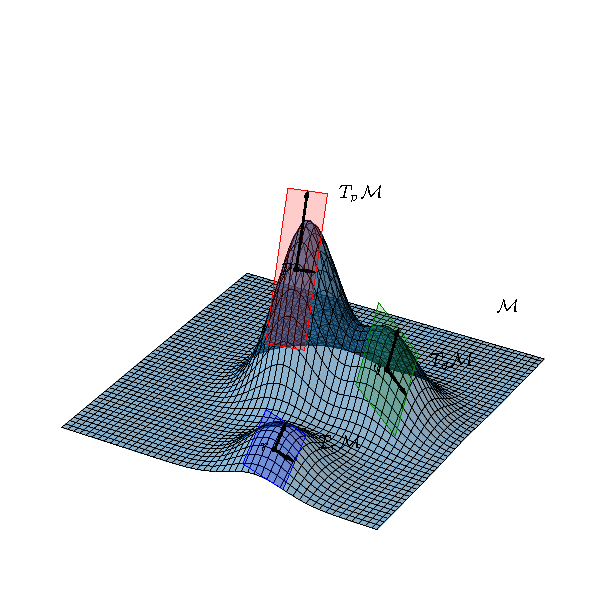
\includegraphics[
			width=4in,
			trim = {0cm 1cm 0cm 3cm},
			clip
			]{images/tangentspaces.pdf}
		\caption{Tangent spaces at points $p$, $q$, and $r$ in an arbitrary manifold $\mcal M$.
			The arrows are the respective basis vectors on the embedding axes.}
		\label{fig:tangentspacesonpoints}
	\end{figure}

	We also say that $\TpM$ is a vector space. The key point here
	is that we need to differentiate $\TpM$ from the manifold $M$ itself.
	$\TpM$ is the space of all vectors that live at $p$, which is not necessarily
	the same thing as $M$.

	This is what makes differential geometry confusing because when we learn
	elementary differential geometry, we often learn it in the context of
	$\R^2$ or $\R^3$. In $\R^2$, the manifold is $\R^2$ itself, so when you get
	a tangent space at a point $p$, call it $T_p\R^2$, which is the space of
	all derivative operators at $p$, then the tangent space is isomorphic to
	$\R^2$ itself. This is why we confuse positions in $\R^2$ with vectors.
	However, in general, that is not the case.

	In this lecture, we will be covering the notion of a tangent vector associated
	with curves on a manifold. Our usual notion of tangency, which is something
	like a tangent line or a tangent plane to curves or surfaces in $\R^2$ or $\R^3$,
	will be recovered as the same notion, but defined more precisely in terms
	of a tangent vector.

	We will draw out a very important distinction between the tangent space
	$\TpM$ and the manifold $\mcal{M}$ itself, which can very often be lumped
	together and confused because $T_p\R^n$ is isomorphic to $\R^n$, which
	is how it is introduced. That is, we have barely any distinction
	between a position vector and a position. For example, say we have a point
	$p$ defined by $(x,y)\in\R^2$. We can then think of a vector
	$(x,y)_p\in T_p\R^2$, and there is really no clear distinction between the two.
	It is important to understand that, in general, manifolds and tangent spaces
	are really different things.

	\subsubsection{Tangent Vector Components}

		We introduce a shorthand when writing down components. In general, a vector
		$v_p$ can always be written in terms of its components
		$v_p^\mu \pdv{}{x^\mu}$, given a chart and the coordinate basis vectors
		coming from that chart. However, these components are just numbers,
		plain real numbers:
		\[
			v_p^\mu\in\R
		\]
		We can compute them easily by having the vector itself $v_p$ act
		on the coordinate functions. That is,
		\begin{equation}
			\label{eq:vectoract}
			v_p^\mu = v_p[x^\mu]
		\end{equation}
		This is a perfectly well-defined operation, since $v_p$ can act on functions,
		and such an operation results in a real number. How can we see that this is true?
		\begin{proof}
			A vector $v_p$ can be written in general as
			\[
				v_p = v_p^\nu \pqty{\pdv{}{x^\nu}}_p
			\]

			We can make this vector act on a coordinate function $x^\mu$:
			\[
				v_p[x^\mu]
				= v_p^\nu \qty(\pdv{}{x^\nu})_p x^\mu
			\]

			Remember how the basis vector operates on functions. To this effect,
			we have
			\[
				v_p[x^\mu]
				= v_p^\nu \qty(\pdv{x^\mu}{x^\nu})_p
			\]

			However, by definition,
			\[
				\pdv{x^\mu}{x^\nu}
				= \tensor{\delta}{^\mu_\nu},
			\]
			therefore
			\[
				v_p[x^\mu]
				= v_p^\nu \tensor{\delta}{^\mu_\nu}
			\]
			Which is just
			\[
				v_p[x^\mu] = v_p^\mu
			\]

			So these components can be obtained by making the vector
			act on the coordinate function.
			\footnote{
				From here on, we use the following convention. For operators, brackets
				$[\cdot]$ indicate that the operator is acting on something, while
				parentheses $(\cdot)$ denote that they depend on something.
			}
		\end{proof}

		We are later going to use this shorthand in our calculations.

		Taking from where we left off in the previous lecture, we discussed
		curves, which are maps from an open interval $I\subseteq\R$ to the manifold,
		i.e.,
		\[
			C:I\to\mcal{M}
		\]

		So if we have a chart, ${x^\mu}$, then a curve is parameterized in $\R^n$ as
		\[
			\psi\circ C \iff x^\mu(t),
			\qquad t\in I\subseteq\R
		\]
		Recall, however, that this is a parameterization. The curve itself is independent
		of the parameterization. Given a curve, we can define a tangent vector.
		If $C(t)$ is a curve, then we define the tangent vector associated with this
		curve as
		\[
			\tau(f) = \eval{\dv{(f\circ C)}{t}}_{t_0}
		\]
		Sometimes, this tangent vector $\tau$ is denoted as
		\begin{equation}
			\label{eq:tauatc}
			\tau = \eval{\pdv{}{t}}_{C(t_0)}
		\end{equation}
		That is, it is a vector at the point $C(t_0)$ that is able to act on functions,
		and it does so precisely as we defined it.

		This is a familiar operation because these are just a set of numbers,
		and we take a derivative of them with respect to $t$. It is a normal derivative
		associated with the point $C(t_0)$.

		Recall that we also previously defined a set of special curves called the
		$x^\mu$ coordinate lines. These are curves which, when mapped by $\psi$
		to $\R^n$, only vary one component while allowing the rest to remain constant.
		It is the image of a curve with parameter $x^\mu$. In effect, since we have
		an association between these sets of points in the image of $C$, $x^\mu$
		becomes a parameter on this curve. It serves as the $t$, so to speak.
		As we vary $x^\mu$ in $\R^n$, the corresponding preimage on the manifold
		also varies. Therefore, we can effectively express this coordinate curve as
		\[
			C(x^\mu)
		\]
		Since $\psi$ is a one-to-one map, its inverse preserves the correspondence
		between curves in the coordinate domain and curves on the manifold. For example,
		if we have $C(x^1)$ and $C(x^2)$, those two curves should be independent
		and will not overlap in the coordinate domain. Each coordinate line in $\R^n$
		will correspond to a different coordinate curve on the manifold, and each
		coordinate serves as a parameter for its corresponding family of curves.
		If this correspondence were not one-to-one, $\psi$ would not be a valid chart.

		Note that we are not just choosing any arbitrary line in $\R^n$. We are choosing
		lines which preserve the other coordinates $x^\nu$, while only varying $x^\mu$.
		For example, consider the polar-coordinate pair $(r,\theta)$. The coordinate
		domain for polar coordinates is a subset of $\R^2$, with
		\[
			r\in[0,\infty),
			\qquad
			\theta\in[0,2\pi).
		\]

		When we map coordinate lines to a manifold, say a ball, we map these lines of
		constant values such that the other coordinates remain fixed while only one
		is allowed to vary. Say we want to map a coordinate line for $\theta$.
		We select a value of $r$, keep it constant, and allow $\theta$ to vary.
		This would be a $\theta$-coordinate line.

		It is not the only $\theta$-coordinate line; there are multiple coordinate
		lines for each coordinate, as long as the other coordinates are held fixed
		and the corresponding coordinate is varied. In this way, we are effectively
		putting a \textit{grid} on the manifold, which corresponds to lines of constant
		values in the coordinate domain.
		\begin{figure}[h]
			\centering
			\includegraphics[width=3in]{polarcoordline.pdf}
			\caption{Coordinate curves of the polar coordinate basis}
			\label{fig:polarcoordline}
		\end{figure}

		Each coordinate is therefore associated with a family of coordinate lines.
		Now that the notion of coordinate curves is understood, and tangent vectors
		are associated with curves, we can then assign tangent vectors to these
		coordinate curves.

		Given an $x^\mu$-coordinate line, with $x^\mu$ as the parameter, it is
		common to denote the tangent vector at a point $p$ as
		\begin{equation}
			\label{eq:tangentvector on a curve}
			\eval{\pdv{}{x^\mu}}_{p} [f]
			= \eval{\pdv{f(x^\mu)}{x^\mu}}_{x^\mu(p)}
		\end{equation}
		with $f$ being an arbitrary function evaluated on the curve.\footnote{
			Recall that when we say $f$, what we really mean is
			$f\circ\psi\inv$, i.e.,
			$f(x) \equiv (f\circ\psi\inv)[x]$.
		}
		We are taking a derivative with respect to the $x^\mu$ parameter.

		Notice that the tangent vector that we wrote in
		(\ref{eq:tangentvector on a curve}) is the same as the definition
		that we used for coordinate basis vectors. This particular definition
		of the tangent vector on a coordinate curve precisely coincides with the
		previous definition of coordinate basis vectors, which we denote in the same way.

		This then implies that coordinate basis vectors are tangent vectors.
		They are tangent vectors associated with the $x^\mu$ coordinate curve.
		They are one and the same.

		We defined vectors previously as simply an abstract notion, but here,
		we recover what we mean by a vector. A coordinate basis vector is simply
		the tangent vector to a coordinate curve, whose components describe the
		rate of change of the coordinates along that curve, and whose direction
		corresponds to increasing $x^\mu$.

		Let's bring this definition a little bit more down to earth. Consider
		$x^\mu(t)$ to be the parametric equations for a curve, i.e., we now use
		coordinates to represent the abstract curve. Let's then consider the action
		of a tangent vector $\tau$ associated with $C(t_0)$ on an arbitrary function $f$:
		\[
			\eval{\pdv{}{t}}_{C(t_0)}f
			= \eval{\dv{f(C(t))}{t}}_{t_0}
		\]

		What we will do is find an expression for this tangent vector that uses the chart.
		We can rewrite this as
		\[
			\eval{\pdv{}{t}}_{C(t_0)}f
			= \eval{\dv{(f\circ\psi\inv\circ\psi\circ C)}{t}}_{t_0}
		\]
		We recall that
		$f\circ\psi\inv:x^\mu\mapsto f\circ\psi\inv(x^\mu)=f(x^\mu)$,
		which is how we represent the function $f$ in coordinates, and
		$\psi\circ C:t\mapsto x^\mu(t)$, which is the parametric form for the curve.
		It looks complicated, but this entire expression is nothing but the following:
		\[
			\eval{\pdv{}{t}}_{C(t_0)}f
			= \eval{\dv{f(x^\mu(t))}{t}}_{t_0}
		\]
		This is just normal calculus. We just use the chain rule:
		\[
			\eval{\pdv{}{t}}_{C(t)} f
			= \eval{\dv{x^\mu}{t}}_{t_0}
				\eval{\pdv{f}{x^\mu}}_{x^\mu(C(t_0))}
		\]
		We rearrange things a bit. Notice that the second term on the right-hand side
		is nothing but (\ref{eq:tangentvector on a curve}). Recall here that
		$p=C(t_0)$. As such, we can write it as the coordinate basis vectors acting on $f$:
		\[
			\eval{\pdv{}{t}}_{C(t_0)} f
			= \eval{\dv{x^\mu}{t}}_{t_0}
				\eval{\pdv{}{x^\mu}}_{x^\mu(C(t_0))} f
		\]
		Since $f$ is arbitrary, we can remove it, and hence we find that
		\begin{equation}
			\label{eq:curve as basis}
			\eval{\pdv{}{t}}_{C(t_0)}
			=
			\eval{\dv{x^\mu}{t}}_{t_0}
			\eval{\pdv{}{x^\mu}}_{x^\mu(C(t_0))}
		\end{equation}

		Recall that this is a tangent vector associated with a curve $C$ at $t_0$,
		and we have now written it down as a linear combination of basis vectors.
		This shows that any tangent vector can be written as a linear combination
		of coordinate basis vectors. Therefore, a tangent vector is a vector in
		the tangent space, represented as a derivation acting on smooth functions.

		Not only that, but the components of the tangent vector are
		\[
			\dv{x^\mu}{t},
		\]
		which is exactly what we understand a tangent vector to be in the usual
		geometric parameterization sense: something analogous to a \textit{velocity},
		the rate of change of the coordinates $x^\mu$ with respect to $t$.

		The distinction here is that what we used to call a tangent vector in a
		mechanical sense is not actually the tangent vector itself; rather,
		$\dot{x}^\mu$ are the components of the tangent vector:
		\[
			\underbrace{\eval{\pdv{}{t}}_p}_{\text{tangent vector}}
			=
			\underbrace{\dv{x^\mu}{t}}_{\text{components}}
			\underbrace{
				\eval{
					\pdv{}{x^\mu}
				}_p
			}_{\text{basis vectors}}.
		\]
		The components require a coordinate system, or a chart. The tangent vector
		itself is independent of the choice of coordinates, but the values of its
		components will change depending on the chart you choose. The tangent vector
		itself does not change; it is a geometric object associated with the curve.
		We are drawing a distinction between coordinate expressions and the object itself.

		So a tangent vector is a vector, which may seem obvious. However, what is
		perhaps more surprising is that directional derivatives themselves are
		tangent vectors.

		\noindent\textit{Exercise: All directional derivatives are tangent vectors.}

		It suffices to show that if you have a derivative operator $v$ acting on
		$f$ at a point $p$, $v[f]$, I can always associate a curve on the manifold
		which passes through $p$, such that we can use that curve to define the same
		tangent vector. Thus, we can always associate a curve with a tangent vector
		at point $p$.
		You should be able to find a curve such that
		\[
			v[f] = \dv{[f(C(t))]}{t},
		\]
		where $v$ is an arbitrary vector acting on an arbitrary $f$. When you have
		shown that, then you have shown that any vector can be associated with some
		curve, and we can do this by invoking the uniqueness of solutions to
		differential equations.

		\begin{question}{Are tangent vectors similar to velocities since it's represented as $\dot{x}^\mu$?}
			The velocity itself, physical velocity, is a tangent vector.

			\hspace{1em}
			In usual physics, we usually refer to
			\[
				\dv{x^\mu}{t}
			\]
			as the velocity. However, the velocity \textit{components} can change
			with a change of chart and coordinates. But the velocity vector itself does not.

			\hspace{1em}
			The tangent vector is not something that depends on $x^\mu$; it is an
			abstract geometric object. $\dot{x}^\mu$ is not the tangent vector;
			it is just the components of the tangent vector. The vector itself is
			a geometric object that precedes the introduction of a chart.

			\hspace{1em}
			Prior to our discussions in this class, the usual way of thinking
			about tangent vectors was through coordinates. But how do we define
			things without coordinates?
			These definitions are precisely what we laid out: vectors are operators
			on functions. If you give a vector a chart, it will have components that
			are identical to how we used to think about tangent vectors.
		\end{question}

		When we do geometry, we are so used to using coordinates, and in this
		form of thinking, we are trying to define objects and geometry that are
		independent of our way of describing them. Geometry is not something
		which depends on how we choose to represent what axes we choose.
		Geometry has to be defined without recourse to coordinates.

		However, as physicists, we always calculate in coordinates for anything practical.
		I am not saying that we are completely going to devalue coordinates;
		we just need to be more careful with them and remember that there is an object
		that precedes the coordinate representation.

		GR is mostly about mindsets, and in this, we take the hierarchy of:
		geometrical objects, basis, components. It's not going to be that hard,
		but it does require a certain frame of mind, because how we define and
		manipulate things in physics is highly dependent on how we interpret and
		think about things.

		If we start with components, GR actually becomes harder. I could have taught
		you GR directly without doing any differential geometry: we could just say
		``these are the equations, these are how they're manipulated,'' and then
		solve the PDEs involved. However, without the foundations given to us by
		differential geometry, it is going to be very difficult to interpret the
		results we obtain.
		You can just compute it, you can put it in \texttt{mathematica} and do the
		calculations, and usually, that's where the bulk of the work comes from.
		But then, once you have a result, how do you think about the result?
		You have to go back to what it means geometrically.

		We always ask that question: What does this mean, geometrically?

		Now, for the rest of the lecture series, and from the previous definitions,
		we denote that there is not going to be any difference between vectors,
		tangent vectors, and derivative operators or derivations. They are all
		one and the same. When you refer to the geometric object with one of those
		names, you refer to all of them.

		You think about the class of curves that is associated with the operator,
		and how a derivation acts on functions.

	\subsubsection{Vector Fields}

		So obviously, tangent vectors at a single point are of limited utility
		in physics. When we do physics, what we really deal with are vector fields.
		So what is a vector field?

		In $\R^n$, a vector field simply means that you define a vector at every point
		in $\R^n$; it is a specification of a vector $v$ for all points $p\in\R^n$.

		A vector field on a manifold works in precisely the same way. It is a
		selection of a vector at every tangent space of a manifold. So if we have
		a manifold $\mcal M$ and take a point $p$, it is associated with a tangent
		space $T_p\mcal M$, and if we take a point $q\in\mcal M$, it is associated
		with a tangent space $T_q\mcal M$.

		At every point, there is going to be a tangent space that can be defined,
		which sort of \textit{sticks out} from the manifold.
		These tangent spaces are vector spaces; however, $\mcal M$ itself is not
		necessarily a vector space.

		Bear in mind that these tangent spaces do not intersect one another.
		We are used to thinking about vectors and planes being embedded in $\R^3$.
		However, in general, there is nothing that exists outside the manifold itself
		that we need to regard as an ambient space.

		Tangent spaces are abstract spaces. There is no ambient space around them
		that the tangent space is a subset of. The only geometric object we are
		assuming is the manifold. There is no intersection between tangent spaces
		at different points.

		We represent tangent spaces as planes because it is a convenient pictorial
		representation; it is easier to visualize. However, there is not really a
		plane in the usual sense. When we say a plane, we think of it as a subset
		of a bigger space. However, a tangent space is not a subset of a bigger
		space; it is simply an abstraction associated with each point on the manifold.
		That's a common misconception, and we wish to differentiate it.

		Moving on, the set of all tangent spaces constitutes the tangent bundle.
		More precisely, the tangent bundle is the disjoint union of all tangent spaces:
		\[
			T\mcal M = \bigcup_p T_p\mcal M.
		\]
		This is called the tangent bundle. A vector field is then a selection
		of a vector at each point, or equivalently, a section of the tangent bundle.

		\begin{definition}{Vector field}
			A vector field $v$ is a section of the tangent bundle $T\mcal M$, which assigns
			a vector $v_p$ for all $p$ in $\mcal{M}$.
		\end{definition}

		Let me explain why that's an appropriate terminology. Let's illustrate it
		with an easy example. Let's say $\mcal M$ is a one-dimensional manifold,
		$\R$. That means you can completely characterize it with one coordinate,
		a line, basically.

		So how would you represent a vector field on a line? How would one represent it?
		Say we have a variable $x$ representing points $p\in\R$. Let's say a vector
		field $v$ is a function of $x$:
		\[
			v(x).
		\]
		Recall that a vector is an operator. It acts on functions and returns
		a real number. A vector field, however, assigns a vector to each point.
		In a coordinate representation on $\R$, this can be described by a
		function of $x$.

		What we really think of then as a vector field is a collection of vectors
		associated with the points in $\R$. The corresponding functions are smooth,
		so the vector field varies smoothly from point to point; this is the usual
		setting of real analysis.
		\begin{figure}[h]
			\centering
			\includegraphics[width=4in, height=2in]{images/vectorfieldRtrad.pdf}
			\caption{A vector field on the $\R$ line}
			\label{fig:vectorfield}
		\end{figure}

		This vector field is just like a normal vector field: it is a bunch of arrows
		throughout. We make a mistake, though, because we think that vectors live
		on $\R$ as arrows. It is how we represent them.

		However, $v(x)$ really lives in a tangent space:
		\[
			v(x)\in T_x\R.
		\]

		However, $v$ does not live on $\R$; it just happens that $T_x\R$ is isomorphic
		to $\R$. What we usually do, then, is simply represent the vector itself
		as existing in $\R$.

		We would like to emphasize the fact that vectors live in tangent spaces,
		and so we represent them on another \textit{axis} instead, similar to how
		we treat complex numbers. We draw arrows like:
		\begin{figure}[h]
			\centering
			\includegraphics[width=4in, height=2in]{images/vectorfildTxR.pdf}
			\caption{Representing a vector field in $T_p\R$ as a different axis}
			\label{fig:vectorfieldTpR}
		\end{figure}

		This is just a different representation of a vector field. What is the
		tangent bundle, then?

		The tangent bundle is the collection of all these tangent spaces. In this
		example, if we represent each tangent space as a separate copy of $\R$,
		the tangent bundle can be visualized as an entire plane. We stitch these
		spaces together as a bundle, and the vector field is then represented as
		a cross-section, or section, of this tangent bundle.

		We can represent a different vector field depending on how we take sections
		of the tangent bundle, and a vector field corresponds to a choice of one
		vector at each point.

	\subsubsection{Connection}

		\begin{question}{Is a tangent bundle one dimension higher than the manifold?}
			It's a tricky question. Strictly speaking, the tangent bundle is not
			defined merely by ``connecting'' tangent spaces, because we have no
			notion of a connection between them from the definitions given so far.
			We \textit{can't} really connect them right now.

			\hspace{1em}
			What we have simply said is that the tangent bundle is a collection
			of tangent spaces, one at each point. There is nothing in what we have
			said so far that allows us to compare or connect objects living on
			different tangent spaces.

			\hspace{1em}
			They are all isomorphic as vector spaces, they have one-to-one correspondences, but there is no natural
			isomorphism or canonical identification between one tangent space and
			another. It requires extra structure. The structure that allows us to
			relate vectors at different points is what we call a \textit{connection},
			which we will discuss soon. Connection is actually what's going to give us curvature.
		\end{question}

		On a manifold, there is no natural notion of vector subtraction or addition
		for vectors living in different tangent spaces. Say you have an arbitrary
		vector $\vb{v}_p$ at a point $p$, living in $\TpM$, and another vector
		$\vb{v}_q$ at a point $q$, living in $T_q\mcal M$. Those two vectors
		are independent of each other: they live in different tangent spaces
		because they are based at two different points on the manifold (refer to Fig. \ref{fig:tangentspacesonpoints})

		You cannot combine them in a natural way. You need to first specify how
		vectors at different points are to be related. You need to provide precise
		instructions for how these vectors are connected. That's why it is called
		a connection.

		A connection is then the additional structure that allows us to compare
		vectors at different points and, together with the appropriate definitions,
		to define curvature. That's what we are getting into in the next few weeks,
		hopefully.

		Now, connection combined with curves gives us the notion of parallel transport.
		We are building the tools needed for us to be able to define and do certain
		things that are taken for granted in physics. We are being very careful and
		laying down the foundations that we will then use in GR.

		If you have a connection and a curve, you have parallel transport. Then,
		given two different points on a curve, you can parallel transport a vector
		from one point to the other. If parallel transport around a closed curve
		fails to return a vector to its original value, i.e., there is a difference
		between the vectors, this is an indication of
		non-zero curvature. We shall discuss this more in the coming weeks.

		\subsubsection*{Exercise Result}
			\begin{proof}
				Let $v$ be a directional derivative at $p\in\mcal M$. Choose a chart
				$(U,\psi)$ around $p$, and write
				\[
					v^\mu = v[x^\mu].
				\]
				Define a curve $C:I\to\mcal M$ by
				\[
					C(t) = \psi\inv\pqty{\psi(p)+t v^\mu e_\mu},
				\]
				for $t$ sufficiently close to $0$. Hence, $C(0) = p$. Writing
				\[
					x^\mu(t) = \psi^\mu(C(t)),
				\]
				we have
				\[
					x^\mu(t)=x^\mu(p)+t v^\mu,
				\]
				and hence
				\[
					\eval{\dv{x^\mu}{t}}_{t=0}=v^\mu.
				\]
				Now, by the chain rule,
				\begin{align}
					\eval{\dv{(f\circ C)}{t}}_{t=0}
					&=
					\eval{\dv{x^\mu}{t}}_{t=0}
					\eval{
						\pdv{(f\circ\psi\inv)}{x^\mu}
					}_{\psi(p)} \\
					&=
					v^\mu
					\eval{
						\pdv{(f\circ\psi\inv)}{x^\mu}
					}_{\psi(p)} \\
					&=
					v^\mu
					\eval{
						\pdv{f}{x^\mu}
					}_{p} \\
					&= v[f].
				\end{align}
				Therefore,
				\[
					v[f]
					=
					\eval{\dv{(f\circ C)}{t}}_{t=0},
				\]
				so $v$ is the tangent vector generated by the curve $C$ at $p$.
				Hence every directional derivative is a tangent vector.
			\end{proof}
	\subsubsection{Physicsal Examples}
		This is all too abstract, no? I\footnote{the author} really can't
		help but lose the sense of groundedness we have on the physical nature of things.
		What we have learned so far is kinda in wooey-magic-abstract land. So
		I have taken it upon myself to find some examples to make these
		abstract concepts more concrete.

		Before we begin, a word on notation. Throughout, we must be careful
		to distinguish several different objects that are too often conflated.
		In particular, we must distinguish the manifold itself, its coordinate
		functions, its parametrization into an ambient space, and the coordinate
		functions of that ambient space.

		Let $\mathcal M$ be an $n$-dimensional manifold, and let
		$U\subseteq\mathcal M$ be a coordinate neighborhood. A coordinate chart
		is a map
		\[
			\psi:U\to\R^n,
		\]
		which assigns $n$ coordinates to each point of $U$. Writing
		\[
			\psi(p)
			=
			\pqty{x^1(p),\ldots,x^n(p)},
		\]
		the functions
		\[
			x^\mu:U\to\R,
			\qquad
			\mu=1,\ldots,n,
		\]
		are the \textit{coordinate functions} on the manifold. They take a
		point $p\in U$ and return its $\mu$-th coordinate. The coordinates
		therefore belong to the description of the manifold itself. They are
		not vectors and they are not the components of a vector.

		Now suppose that $\mathcal M$ is embedded in an $m$-dimensional
		ambient space, which we take to be $\R^m$. Let the ambient coordinates
		be denoted by $X^\nu$, with
		\[
			X^\nu:\R^m\to\R,
			\qquad
			\nu=1,\ldots,m.
		\]
		These ambient coordinate functions describe points from the perspective
		of the surrounding space.

		If the manifold is embedded through a parametrization
		\[
			\vb{r}:V\subseteq\R^n\to\R^m,
		\]
		then its components are the ambient coordinates evaluated on the
		parametrized point:
		\[
			\vb{r}(x^1,\ldots,x^n)
			=
			\bigl(
				X^1(x^1,\ldots,x^n),
				\ldots,
				X^m(x^1,\ldots,x^n)
			\bigr).
		\]
		More precisely, the functions appearing here are the compositions
		$X^\nu\circ\vb r$, with the composition conventionally suppressed.

		Let $\{\vb e_\nu\}$ denote the standard basis of the ambient space,
		\[
			\vb e_\nu=\pdv{}{X^\nu}.
		\]
		Then the position vector of the embedded point may be written as
		\[
			\vb r
			=
			X^\nu\vb e_\nu,
		\]
		or, as a function of the intrinsic coordinates,
		\[
			\vb r(x^\mu)
			=
			X^\nu(x^\mu)\vb e_\nu.
		\]

		The chart $\psi$ and the parametrization $\vb r$ are inverse maps on
		the corresponding coordinate patch. If
		\[
			u=\psi(p)
			=
			\pqty{x^1(p),\ldots,x^n(p)},
		\]
		then
		\[
			\vb r(u)=p.
		\]
		Thus,
		\[
			\vb r\circ\psi=\operatorname{id}_U.
		\]
		Conversely,
		\[
			\psi\circ\vb r=\operatorname{id}_{V}
		\]
		when $\vb r$ is the parametrization associated with the chart.

		The distinction is therefore:
		\begin{itemize}
			\item $\mathcal M$ is the manifold itself.
			\item $x^\mu$ are the coordinate functions on $\mathcal M$.
			\item $X^\nu$ are the coordinate functions of the ambient space.
			\item $\vb r$ is the parametrization or embedding map which
			      realizes the manifold as a subset of the ambient space.
		\end{itemize}

		The relationship between the intrinsic and ambient descriptions becomes
		particularly useful when constructing a basis for the tangent space.
		The coordinate basis on $\mathcal M$ is
		\[
			\left\{
				\partial_\mu
			\right\}
			=
			\left\{
				\frac{\partial}{\partial x^\mu}
			\right\}.
		\]
		These are tangent vectors to the manifold. Under the embedding, their
		images in the ambient tangent space are obtained by differentiating
		the embedding:
		\[
			\pdv{\vb r}{x^\mu}
			=
			\pdv{X^\nu}{x^\mu}
			\pdv{}{X^\nu}
			=
			\pdv{X^\nu}{x^\mu}\vb e_\nu.
		\]
		Note that this operation also just results in itself. By the chain rule, we find that $\p_\mu\vb{r}\equiv \p_\mu$. This is an important property we will use later.
		\begin{equation}
			\label{eq:vector-embed-eqiuvalence}
			\pdv{\vb{r}}{x^\mu}
			=
			\pdv{X^\nu}{x^\mu}\pdv{}{X^\nu}
			=
			\pdv{}{x^\mu}.
		\end{equation}
		Hence, we recover the coordinate basis vector when differentiating the
		embedding with respect to its corresponding coordinate.

		Thus, the Jacobian
		\[
			\pdv{X^\nu}{x^\mu}
		\]
		gives the components of the embedded tangent basis vectors
		$\partial\vb r/\partial x^\mu$ with respect to the ambient basis
		$\{\vb e_\nu\}$. In particular, the tangent basis of the embedded
		manifold is
		\[
			\left\{
				\pdv{\vb r}{x^\mu}
			\right\}.
		\]

		With this distinction established, we can finally look at some concrete
		examples with more explicit operations and presentation.

		\begin{enumerate}[(1)]
			\item The Cartesian plane ($\R^2$)

				Take, for example, a flat $2$D manifold parameterized by its
				intrinsic coordinate parameters $u,v$. We can embed this manifold
				in the Cartesian plane through the parametrization
				\[
					\vb{r}(u,v)
					=
					\bigl(x(u,v),y(u,v)\bigr),
				\]
				where we define
				\[
					x(u,v)=u,
					\qquad
					y(u,v)=v.
				\]
				Thus,
				\[
					\vb{r}(u,v)=(u,v).
				\]

				To find the coordinate basis vectors at a point
				$p=\vb{r}(u,v)$, we take the partial derivatives of the
				parametrization with respect to each intrinsic coordinate:
				\[
					\partial_u\vb{r}
					=
					\pdv{\vb{r}}{u},
					\qquad
					\partial_v\vb{r}
					=
					\pdv{\vb{r}}{v}.
				\]
				Since the components of $\vb{r}$ are $x$ and $y$, we have
				\begin{align*}
					\partial_u\vb{r}
					&=
					\pqty{
						\pdv{x}{u},
						\pdv{y}{u}
					}
					=
					\pqty{
						\pdv{u}{u},
						\pdv{v}{u}
					}
					=
					(1,0),
					\\
					\partial_v\vb{r}
					&=
					\pqty{
						\pdv{x}{v},
						\pdv{y}{v}
					}
					=
					\pqty{
						\pdv{u}{v},
						\pdv{v}{v}
					}
					=
					(0,1).
				\end{align*}

				Therefore, the coordinate basis is
				\[
					\left\{
						\partial_u,\partial_v
					\right\}
					=
					\left\{
						(1,0),(0,1)
					\right\}.
				\]
				But since $u=x$ and $v=y$, these are precisely the Cartesian
				basis vectors:
				\[
					{
						\partial_u=\partial_x,
						\qquad
						\partial_v=\partial_y.
					}
				\]
				In other words, because the intrinsic coordinates $(u,v)$ are
				identical to the ambient Cartesian coordinates $(x,y)$, the
				intrinsic coordinate basis of the manifold coincides with the
				usual Euclidean Cartesian basis.

				Notice, then, that the components of the cartesian basis are 
				\[
					\pdv{}{x}\vb{r} = (1,0) \qquad \pdv{}{y} \vb{r} = (0,1)
				\]
				These are simply the components of the usual elementary Cartesian
				basis we know from elementary differential geometry. This is where the 
				\textit{sense} of being a column matrix being isomorpic to a vector comes 
				from. The matrix elements comes from differentiating the coordinates of 
				the parameterization $\vb{r} = X^\nu$, with the coordinate basis for the manifold
				$x^\mu$. The $\nu$-th component of the basis therefore is

				\[
					(\p_\mu \vb{r})^\nu = \pdv{X^\nu}{x^\mu} 
				\]

				Therefore, for a parametrization $\vb{r} = (x,y)$ which is equivalent
				to a Euclidean plane, we define that the components of the basis vectors are
				\[
					\vb{e}_x = \p_x \vb{r} = \bmqty{
						1\\0
					}  
					\qquad \vb{e}_y = \p_y\vb{r} = 
					\bmqty{
						0\\1
					} 
				\]

				The components therefore, are what we usually refer in physics 
				as vectors. 

				\begin{remark}
				    We remark that in usual physics, what we call a vector
					\[
						\vb{v} = \bmqty{
							v^1\\v^2\\v^3
						} 
					\]
					is not really the vector, but its instead its components.

					The actual vector is $\vb{v} = v^\mu \p_\mu$, but we use the 
					components and the actual vector interchangably. What we call the 
					elementary basis vectors $\vb{e}_x$, $\vb{e}_y$, and so on, the matrices
					\[
						\vb{e}_x = \bmqty{
							1&0&0
						}^\top \qquad \vb{e}_y = \bmqty{
							0&1&0
						}^\top
					\]
					is not the vector itself, but the components of the vector, $(\vb{e}_x)^\nu$.
					The actual vector is $\vb{e}_x = \partial_x$,
					whose components in the coordinate basis $\{\partial_x, \partial_y, \partial_z\}$
					are $(1, 0, 0)$.
					A vector whose components are $(1, 0, 0)$ is
					\[
						\vb{v} = v^\mu \partial_\mu = 1 \cdot \partial_x + 0 \cdot \partial_y + 0 \cdot \partial_z
						= \partial_x.
					\]
					However, we can kinda cross over this by doing what I call the \textit{ambient representation}.
					From earlier, we got a result that is 
					\[
						\p_\mu \vb{r} \equiv \p_\mu
					\]
					That is, when a coordinate basis acts on an embedding, it sort of recovers itself. That is not 
					exactly true, but it shows that a the result of a basis acting on an embedding, and the basis
					itself, are isomorphic, i.e., $\p_x \vb{r}\equiv \p_x$ or $\p_y \vb{r} \equiv \p_y$. This is how
					we recover the introductory vector physics representation of a basis vector. 
				\end{remark}

			\item An abstract $1$D manifold embedded in $\R^2$

				A $1$D manifold is a space in which one coordinate is sufficient
				to specify a point locally. Let the coordinate on the manifold
				be $t$, so that
				\[
					t:\mathcal M\to\R.
				\]
				We can embed this $1$D manifold into $\R^2$ through
				\[
					\vb{r}(t)
					=
					\bigl(
						x(t),y(t)
					\bigr).
				\]
				Here $x$ and $y$ are the ambient coordinate functions, in $\R^2$ cartesian coordinates. The
				parameter $t$, on the other hand, is the coordinate on the
				manifold itself.

				The coordinate basis of the tangent space is simply
				\[
					\left\{
						\partial_t
					\right\}.
				\]
				As an ambient vector, this basis vector is obtained by
				differentiating the embedding:
				\[
					\partial_t\vb{r}
					=
					\pdv{x}{t}\vb{e}_x
					+
					\pdv{y}{t}\vb{e}_y.
				\]
				Equivalently,
				\[
					\partial_t\vb{r}
					=
					\pqty{
						\dv{x}{t},
						\dv{y}{t}
					}
				\]

				An arbitrary tangent vector is therefore
				\[
					v=v^t\partial_t.
				\]
				As an ambient vector (the tangent vector acting on an ambient embedding), we can express this explicitly as components.
				\[
					v[\vb{r}]
					=
					v^t\partial_t\vb{r}
					=
					v^t
					\left(
						\dv{x}{t}
						,
						\dv{y}{t}
					\right).
				\]

				Notice what happened here. The manifold has only one intrinsic
				direction, represented by $\partial_t$, even though its embedding
				lives in a two-dimensional ambient space. The vector therefore
				has one intrinsic component $V^t$, while its representation in
				the ambient space has two components.

			\item An abstract $2$D manifold embedded in $\R^3$

				Now consider a $2$D manifold with coordinates $(u,v)$. We can
				embed it into $\R^3$ through
				\[
					\vb{r}(u,v)
					=
					\bigl(
						x(u,v),
						y(u,v),
						z(u,v)
					\bigr).
				\]
				The manifold has two coordinate basis vectors,
				\[
					\left\{
						\partial_u,\partial_v
					\right\}.
				\]
				To find their components in the ambient space, we differentiate
				the components of the embedding:
				\[
					\partial_u\vb{r}
					=
					\pqty{
						\pdv{x}{u},
						\pdv{y}{u},
						\pdv{z}{u}
					},
					\qquad
					\partial_v\vb{r}
					=
					\pqty{
						\pdv{x}{v},
						\pdv{y}{v},
						\pdv{z}{v}
					}.
				\]

				We will refer to these component representations in the same
				way that vectors are usually written in elementary physics. Recall
				the result we got earlier, that a basis acting on an embedding 
				is equivalent to itself (or to some extent)
				\[
				\p_\mu \vb{r} \equiv \p_\mu
				\]
				it is not the same, obviously, but it is \textit{isomorphic}, which
				allows us to write vectors in the more traditional and intuitive
				way of thinking about them.

				From this, we can show that, in example (1), we have the result.
				\[
					\p_x \vb{r} = \vb{e}_x = \bmqty{
						1\\0\\0
					} \qquad 
					\p_y \vb{r} = \vb{e}_y = \bmqty{
						0\\1\\0
					} \qquad 
				\]
				We can instead get rid of the operation on the embedding, and just 
				represent the vectors precisely as their ambient representation. This
				is a heuristic, a shorthand, it is not physical at all. However, it allows us to think 
				of a vector in the usual and intuitive way it is presented in elementary vector physics.
				That is, we define that $\p_\mu \equiv \p_\mu \vb{r}$, for a certain
				ambient representation of an embedding $\vb{r}$. Hence, we \textit{define}
				that
				\[
					\p_x \equiv \vb{e}_x = \bmqty{
						1\\0\\0
					} \qquad 
					\p_y \equiv \vb{e}_y = \bmqty{
						0\\1\\0
					} \qquad 
				\]
				
				Thus, although $\partial_u$ and $\partial_v$ are the actual
				tangent vectors, we may write their ambient representations as
				\[
					\partial_u
					=
					\pqty{
						\pdv{x}{u},
						\pdv{y}{u},
						\pdv{z}{u}
					},
					\qquad
					\partial_v
					=
					\pqty{
						\pdv{x}{v},
						\pdv{y}{v},
						\pdv{z}{v}
					}.
				\]

				An arbitrary tangent vector $V$ in the ambient space is\footnote{This is not really a vector, this is the result of a vector acting on an embedding, $V[\vb{r}]$, but we shall refer to it as a vector for now. It's a shorthand. This is where we also get $\p_\mu \vb{r}\equiv \p_\mu$, what we usually call a vector is instead $v[\vb{r}] = v^\mu \p_\mu\vb{r}$}.
				\[
					V
					=
					V^u\partial_u+V^v\partial_v.
				\]
				Therefore, in terms of its ambient components,
				\[
					V
					=
					V^u
					\pqty{
						\pdv{x}{u},
						\pdv{y}{u},
						\pdv{z}{u}
					}
					+
					V^v
					\pqty{
						\pdv{x}{v},
						\pdv{y}{v},
						\pdv{z}{v}
					},
				\]
				or
				\[
					V
					=
					\pqty{
						V^u\pdv{x}{u}+V^v\pdv{x}{v},
						V^u\pdv{y}{u}+V^v\pdv{y}{v},
						V^u\pdv{z}{u}+V^v\pdv{z}{v}
					}.
				\]

				Thus, the vector has only two independent components,
				$V^u$ and $V^v$, even though its representation in the
				three-dimensional ambient space has three components. The
				three ambient components are constrained by the fact that the
				vector must remain tangent to the embedded surface.

				Thus, we are not really showing what the vector really is, we 
				are showing how it would look like in the ambient space $\R^3$,
				which is much more intuitive and physical for us.


			\item The unit circle

				Consider the unit circle embedded in $\R^2$, parameterized by
				the intrinsic coordinate $\theta$:
				\[
					\vb{r}(\theta)
					=
					\bigl(
						\cos\theta,\sin\theta
					\bigr).
				\]
				The circle has one coordinate basis vector,
				\[
					\left\{
						\partial_\theta
					\right\}.
				\]
				Differentiating the components of the embedding gives
				\[
					\partial_\theta\vb{r}
					=
					\pqty{
						-\sin\theta,
						\cos\theta
					}.
				\]
				Thus, referring to the vector by its usual elementary-physics
				component representation, we write
				\[
					\partial_\theta
					=
					\pqty{
						-\sin\theta,
						\cos\theta
					}.
				\]

				An arbitrary tangent vector is
				\[
					V=V^\theta\partial_\theta.
				\]
				Its ambient components are therefore
				\[
					V
					=
					V^\theta
					\pqty{
						-\sin\theta,
						\cos\theta
					}
					=
					\pqty{
						-V^\theta\sin\theta,
						V^\theta\cos\theta
					}.
				\]

				Although the vector is represented by two components in the
				ambient plane, it has only one independent component, $V^\theta$,
				because the circle is a $1$D manifold.
			\item Polar coordinates

				Consider the Euclidean plane $\R^2$, parameterized by the
				polar coordinates $(r,\theta)$. We can regard the plane as a
				$2$D manifold $\mathcal M$ with coordinate functions
				\[
					r:\mathcal M\to\R,
					\qquad
					\theta:\mathcal M\to\R.
				\]
				We embed this manifold into $\R^2$ through
				\[
					\vb{r}(r,\theta)
					=
					\bigl(
						x(r,\theta),
						y(r,\theta)
					\bigr),
				\]
				where
				\[
					x(r,\theta)=r\cos\theta,
					\qquad
					y(r,\theta)=r\sin\theta.
				\]
				Thus,
				\[
					\vb{r}(r,\theta)
					=
					\bigl(
						r\cos\theta,
						r\sin\theta
					\bigr).
				\]

				The coordinate basis of the manifold is
				\[
					\left\{
						\partial_r,\partial_\theta
					\right\}.
				\]
				To find their components in the ambient Cartesian space, we
				differentiate the components of the embedding:
				\[
					\partial_r\vb{r}
					=
					\pqty{
						\pdv{x}{r},
						\pdv{y}{r}
					}
					=
					\pqty{
						\cos\theta,
						\sin\theta
					},
				\]
				and
				\[
					\partial_\theta\vb{r}
					=
					\pqty{
						\pdv{x}{\theta},
						\pdv{y}{\theta}
					}
					=
					\pqty{
						-r\sin\theta,
						r\cos\theta
					}.
				\]

				Once again, we refer to the component representations 
				in the same way as elementary vector physics.
				Thus, the coordinate basis vectors have the ambient
				representations
				\[
					\partial_r = \vb{e}_r
					=
					\pqty{
						\cos\theta,
						\sin\theta
					},
					\qquad
					\partial_\theta = \vb{e}_\theta
					=
					\pqty{
						-r\sin\theta,
						r\cos\theta
					}.
				\]

				An arbitrary tangent vector is
				\[
					V
					=
					V^r\partial_r
					+
					V^\theta\partial_\theta.
				\]
				Therefore, its ambient Cartesian components are
				\[
					V
					=
					V^r
					\pqty{
						\cos\theta,
						\sin\theta
					}
					+
					V^\theta
					\pqty{
						-r\sin\theta,
						r\cos\theta
					}.
				\]
				Combining the components gives
				\[
					V
					=
					\pqty{
						V^r\cos\theta
						-
						rV^\theta\sin\theta,
						\,
						V^r\sin\theta
						+
						rV^\theta\cos\theta
					}.
				\]

				Thus, the vector has two independent components, $V^r$ and
				$V^\theta$, corresponding to the two intrinsic directions of
				the manifold. Its representation in the ambient Cartesian
				space also has two components, but these are related to
				$V^r$ and $V^\theta$ through the coordinate transformation.

			\item The unit sphere

				Consider the unit sphere $S^2$ embedded in $\R^3$. Using spherical
				coordinate functions $(\theta,\phi)$ that describe the surface,
				its embedding is
				\[
					\vb{r}(\theta,\phi)
					=
					\bigl(
						\sin\theta\cos\phi,
						\sin\theta\sin\phi,
						\cos\theta
					\bigr).
				\]
				The coordinate basis of the sphere is
				\[
					\left\{
						\partial_\theta,\partial_\phi
					\right\}.
				\]
				Differentiating the components of the embedding gives
				\[
					\partial_\theta\vb{r}
					=
					\pqty{
						\cos\theta\cos\phi,
						\cos\theta\sin\phi,
						-\sin\theta
					},
				\]
				and
				\[
					\partial_\phi\vb{r}
					=
					\pqty{
						-\sin\theta\sin\phi,
						\sin\theta\cos\phi,
						0
					}.
				\]

				Referring to them in the same way as elementary vector physics\footnote{I must reiterate this enough. This is a heuristic, a tool, that relates the abstract vector to how it is usually presented in introductory physics to make it more intuitive. Do not confuse the elementary vector representation to what the actual vector (geometric object) is. They are not the same thing.}
				Thus, the two coordinate basis vectors have the ambient
				representations
				\begin{align*}
					\partial_\theta
					&=
					\pqty{
						\cos\theta\cos\phi,
						\cos\theta\sin\phi,
						-\sin\theta
					}\\
					\partial_\phi
					&=
					\pqty{
						-\sin\theta\sin\phi,
						\sin\theta\cos\phi,
						0
					}
				\end{align*}
				An arbitrary tangent vector is
				\[
					V
					=
					V^\theta\partial_\theta
					+
					V^\phi\partial_\phi.
				\]
				Therefore, its ambient components are
				\[
					V
					=
					\bmqty{
						V^\theta\cos\theta\cos\phi
						-
						V^\phi\sin\theta\sin\phi\\
						V^\theta\cos\theta\sin\phi
						+
						V^\phi\sin\theta\cos\phi\\
						-V^\theta\sin\theta
					}
				\]

				Thus, although the vector is represented by three components
				in the ambient space, it has only two independent components,
				$V^\theta$ and $V^\phi$, because it is tangent to a $2$D manifold.
			\item A $2$D manifold as a surface graph

				Consider the surface
				\[
					\vb{r}(x,y)
					=
					\qty(
						x,y,z(x,y)
					).
				\]
				Here the intrinsic coordinates are $x$ and $y$, while the
				ambient coordinates are $(X,Y,Z)$, with
				\[
					X=x,
					\qquad
					Y=y,
					\qquad
					Z=z(x,y).
				\]

				The intrinsic coordinate basis is
				\[
					\left\{
						\partial_x,\partial_y
					\right\}.
				\]
				To find their components in the ambient space, we differentiate
				the components of the embedding:
				\[
					\partial_x\vb{r}
					=
					\pqty{
						\pdv{X}{x},
						\pdv{Y}{x},
						\pdv{Z}{x}
					}
					=
					\pqty{
						1,
						0,
						\pdv{z}{x}
					},
				\]
				and
				\[
					\partial_y\vb{r}
					=
					\pqty{
						\pdv{X}{y},
						\pdv{Y}{y},
						\pdv{Z}{y}
					}
					=
					\pqty{
						0,
						1,
						\pdv{z}{y}
					}.
				\]
				Referring to them in elementary vector representation, we have:
				\[
					\partial_x
					=
					\pqty{
						1,
						0,
						\pdv{z}{x}
					},
					\qquad
					\partial_y
					=
					\pqty{
						0,
						1,
						\pdv{z}{y}
					}.
				\]

				An arbitrary tangent vector is
				\[
					V
					=
					V^x\partial_x
					+
					V^y\partial_y.
				\]
				Therefore, its ambient components are
				\[
					V
					=
					V^x
					\pqty{
						1,
						0,
						\pdv{z}{x}
					}
					+
					V^y
					\pqty{
						0,
						1,
						\pdv{z}{y}
					}.
				\]
				Combining the components gives
				\[
					V
					=
					\pqty{
						V^x,
						V^y,
						V^x\pdv{z}{x}
						+
						V^y\pdv{z}{y}
					}.
				\]
		\end{enumerate}

		From all this, we gather how we can represent vectors (the geometric abstract object) 
		which are operators, in a more physical and intuitive manner, which are column matrices. We therefore 
		arrive with the following realization:
		\begin{definition}{Traditional vectors}
		    The \textbf{traditional vector}, which is what is usually taught in introductory physics, is not 
			really a vector. \textbf{A vector is a derivation. What we usually call a vector (traditional), is the vector (derivation)
			acting on an ambient embedding space}.
		\end{definition}
		This \textit{ambient representation}, which removes the 
		notion of the embedding, is not fundamental.
		It will not be present in the rest of this work. Think of it simply
		as a shorthand, a heuristic that will allow you to quickly think about and recover
		the familar picture of the traditional vector from its geometric formulation. This is not rigorous by itself,
		I just discovered this on my own by fucking around with the math of actual examples
		(which is then validated by further reading). It's a practical method, but really, this isn't rigourous at all. A rigourous formulation
		would be to show a vector as acting on embedding coordinate functions. However it 
		allows for a more physical representation of the abstract spaces, so it's fine by me.
	\newpage
